\documentclass[12pt]{article}
\usepackage{graphicx}
\usepackage{listings}
\usepackage{amsmath}

\title{Lab1}
\author{Ba12-104 Nguyen Ngoc Lan}
\date{\today}

\begin{document}

\maketitle

\section{Protocol Design}
The file transfer protocol follows these steps:
\begin{enumerate}
    \item The server listens on a specific port for incoming connections.
    \item The client establishes a connection with the server.
    \item The client reads the file in chunks and sends it to the server.
    \item The server writes the received chunks to a file.
    \item The connection is closed.
\end{enumerate}

\begin{figure}[h]
    \centering
    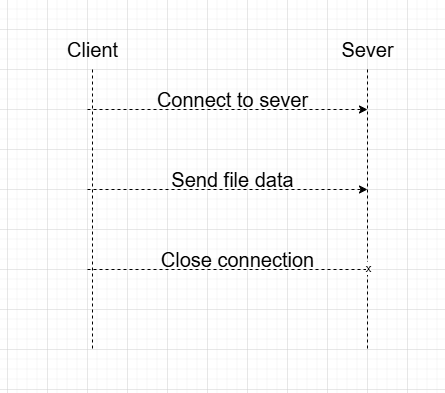
\includegraphics[width=0.8\textwidth]{1.png}
    \caption{Protocol Design Flow}
    \label{fig:protocol}
\end{figure}

\section{System Organization}
The system comprises two components:
\begin{enumerate}
    \item \textbf{Server:} Accepts incoming connections and writes the received data to a file.
    \item \textbf{Client:} Connects to the server and sends the file data.
\end{enumerate}

\begin{figure}[h]
    \centering
    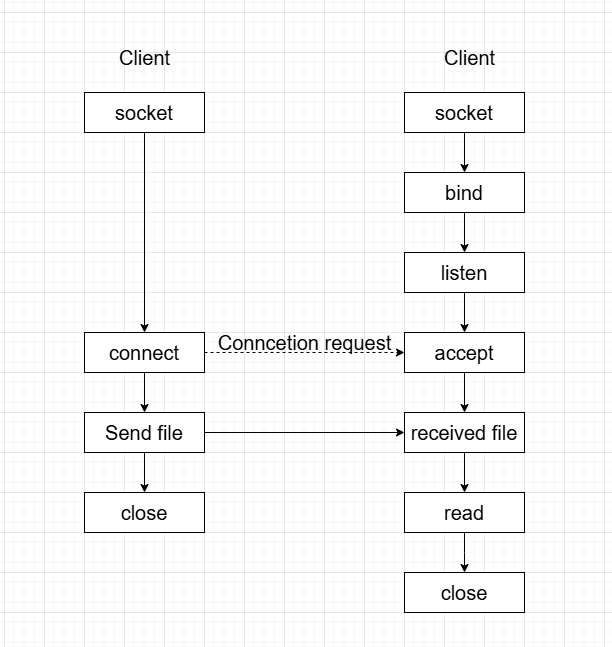
\includegraphics[width=0.8\textwidth]{2.png}
    \caption{Client-Server Architecture}
    \label{fig:architecture}
\end{figure}

\section{Implementation}
The file transfer is implemented using Python sockets. Below are the key snippets:

\subsection{Client Code}
\begin{lstlisting}[language=Python, caption=Client code: send\_file()]
import socket

def send_file(server_host, server_port, file_path):
    client_socket = socket.socket(socket.AF_INET, socket.SOCK_STREAM)
    client_socket.connect((server_host, server_port))
    print(f"Connected to {server_host}:{server_port}")
    
    with open(file_path, 'rb') as file:
        while chunk := file.read(1024):
            client_socket.send(chunk)
    
    print("File sent successfully!")
    client_socket.close()

if __name__ == "__main__":
    send_file("192.168.12.253", 6969, "transferfile.txt")
\end{lstlisting}

\subsection{Server Code}
\begin{lstlisting}[language=Python, caption=Server code: start\_server()]
import socket

def start_server(host='0.0.0.0', port=6969):
    server_socket = socket.socket(socket.AF_INET, socket.SOCK_STREAM)
    server_socket.bind((host, port))
    server_socket.listen(1)
    print(f"Server listening on {port}...")
    
    conn, addr = server_socket.accept()
    print(f"Connected by {addr}")
    
    with open("received_file.txt", 'wb') as file:
        while chunk := conn.recv(1024):
            file.write(chunk)
    
    print("File received successfully!")
    conn.close()
    server_socket.close()

if __name__ == "__main__":
    start_server()
\end{lstlisting}

\end{document}
